Dans tout ce chapitre, on considère \({(X_n)}_{n\geq 1}\) 
une suite de variables aléatoires réelles (ou complexes)
définies sur un espace probabilisé \((\Omega, \scr F, \bb P)\)
et une variable aléatoire \(X\) réelle (ou complexe).

\section{Différents modes de convergence} % 3.1

\subsection{Convergences presque sûre et probabilité} % 3.1.1

\begin{definition}
    On dit que \(X_n\) converge \defemph{presque sûrement} vers
    \(X\) et on note \(X_n \cvpsn X\),
    si
    \begin{equation*}
        \bb P(X_n \underset{n\to\infty}{\longrightarrow} X)
        = \bb P\left(\left\{\omega \in \Omega \mid X_n(\omega) \underset{n\to\infty}{\longrightarrow} X(\omega)\right\}\right)
        = 1.
    \end{equation*}
\end{definition}

\begin{remark}\,
    \begin{enumerate}
        \item Cela correspond à la convergence presque partout pour la
        mesure de probabilité \(\bb P\).

        \item Si \(X_n \cvpsn X\)
        et si \(h: \R \to \R\) est une fonction continue, alors
        \(h(X_n) \cvpsn h(X)\). En particulier, si
        \(X_n \cvpsn X\) et \(Y_n \cvpsn Y\), alors
        \begin{equation*}
            aX_n + bY_n \cvpsn aX + bY,\quad a, b \in \R.
        \end{equation*}
        et
        \begin{equation*}
            X_n Y_n \cvpsn XY.
        \end{equation*}
    \end{enumerate}
\end{remark}

\begin{definition}
    On dit que \({(X_n)}_{n\geq 1}\) converge \defemph{en probabilité} vers
    \(X\) si
    \begin{equation*}
        \forall \varepsilon > 0,\bb P(\n{X_n - X} \geq \varepsilon) \underset{n\to\infty}{\longrightarrow} 0.
    \end{equation*}
    On note alors \(X_n \cvp X\).

    Cela signifie que la probabilité que \(X_n\) s'écarte de \(X\)
    d'un écart supérieur à \(\varepsilon\) tend vers 0 lorsque
    \(n\) tend vers l'infini.
\end{definition}

\begin{example}
    \ptr{} On considère \(X_n\sim \mathcal E(n)\)
    % insert a graph here of the exponential distribution for n = 1, 2, 3, 4
    % representation de densites f_n de X pour n = 1...4, f_n(x) = n e^{-nx}
    \begin{center}
        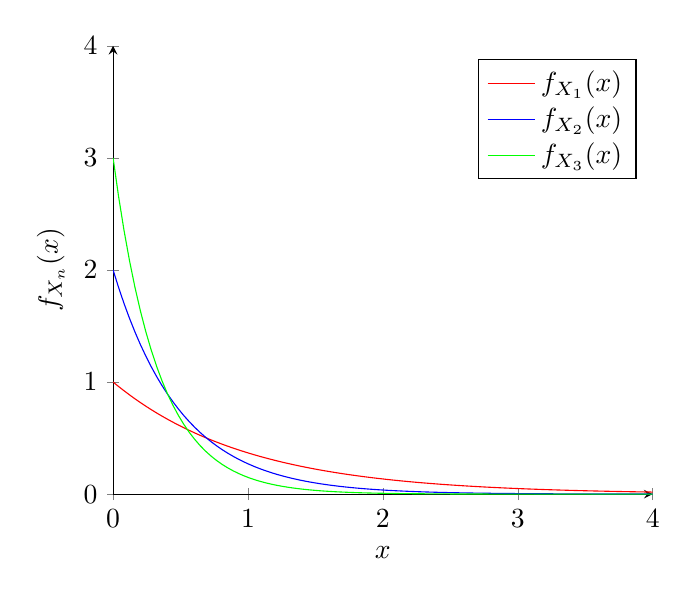
\begin{tikzpicture}
            \begin{axis}[
                axis lines = left,
                xlabel = \(x\),
                ylabel = {\(f_{X_n}(x)\)},
                xmin = 0,
                xmax = 4,
                ymin = 0,
                ymax = 4,
                legend pos = north east,
            ]
            \addplot [
                domain=0:4,
                samples=100,
                color=red,
            ]
            {exp(-x)};
            \addlegendentry{\(f_{X_1}(x)\)}
            \addplot [
                domain=0:4,
                samples=100,
                color=blue,
            ]
            {2*exp(-2*x)};
            \addlegendentry{\(f_{X_2}(x)\)}
            \addplot [
                domain=0:4,
                samples=100,
                color=green,
            ]
            {3*exp(-3*x)};
            \addlegendentry{\(f_{X_3}(x)\)}
            \end{axis}
        \end{tikzpicture}
    \end{center}
    Regardons \(\bb P(\n{X_n} \geq \varepsilon)\):
    \begin{equation*}
        \begin{aligned}
            \bb P(\n{X_n} \geq \varepsilon)
            &= \bb P(X_n \geq \varepsilon)\\
            &= \int_\varepsilon^{+\infty} n e^{-nx} \der x\\
            &= \ff{-e^{-nx}}_\varepsilon^{+\infty}\\
            &= e^{-n\varepsilon}.
        \end{aligned}
    \end{equation*}
    Donc \(X_n \cvpn 0\).

    On peut montrer que \(X_n \cvpsn 0\) (en TD).
\end{example}

\begin{proposition}
    Si \(X_n \cvpsn X\), alors \(X_n \cvp X\).
\end{proposition}

\begin{proof}
    Soit \(\varepsilon > 0\). On a
    \begin{equation*}
            \bb P(\n{X_n - X} \geq \varepsilon)
            = \bb E[\color{red}\underbrace{\color{black}\one_{\n{X_n - X} \geq \varepsilon}}_{f_n\underset{n\to\infty}{\to}0-\text{p.p.}}\color{black}]
    \end{equation*}
    Comme \(\n{f_n}\leq 1\) qui est intégrable, le théorème de convergence
    dominée donne
    \begin{equation*}
        \bb P(\n{X_n - X} \geq \varepsilon)
        = \bb E[\lim_{n\to\infty} \one_{\n{X_n - X} \geq \varepsilon}]
        = 0.
    \end{equation*}
\end{proof}

\begin{example}[Réciproque fausse]
    On considère \({(X_n)}_{n\geq 1}\) une suite de variables aléatoires
    de loi
    \begin{equation*}
        \bb P(X_n = n) = \frac{1}{n},\quad\text{et}\quad \bb P(X_n = 0) = 1 - \frac{1}{n}.
    \end{equation*}
    Soit \(\varepsilon >0\). Alors
    \begin{equation*}
        \bb P(\n{X_n} \geq \varepsilon)
        \leq \frac1n \underset{n\to\infty}{\longrightarrow} 0.
    \end{equation*}
    donc \(X_n \cvpn 0\).

    Supposons que les \({(X_n)}_{n\geq 1}\) sont indépendantes.
    Les événements \(A_n = \{X_n = n\}\) sont indépendants
    et vérifient
    \begin{equation*}
        \begin{aligned}
            \sum_{n=1}^{+\infty} \bb P(A_n) 
            &= \sum_{n=1}^{+\infty} \bb P(X_n = n)\\
            &= \sum_{n=1}^{+\infty} \frac{1}{n}\\
            &= +\infty.
        \end{aligned}
    \end{equation*}
    Donc par Borel-Cantelli, on a
    \begin{equation*}
        \bb P(\limsup_{n\to\infty} A_n) = 1.
    \end{equation*}
    Donc avec probabilité 1, \(X_n\) prend la valeur \(n\) 
    une infinité de fois. Donc avec probabilité 1, 
    \({(X_n)}_{n\geq 1}\) ne converge pas vers 0.
    Donc \({(X_n)}_{n\geq 1}\) ne converge pas presque sûrement.
\end{example}

\begin{proposition}[Loi faible des grands nombres]
    Soit \({(X_n)}_{n\geq 1}\) une suite de variables aléatoires
    réelles dans \(\mathcal L^2(\Omega, \scr F, \bb P)\). On
    suppose que les \(X_n\) sont indépendantes et identiquement
    distribuées (c'est-à-dire de même loi, i.i.d.\ en abrégé).

    On note \(\mu\) leur espérance: \(\mu = \bb E[X_1]\). On
    pose \(S_n = X_1 + \cdots + X_n\). Alors
    \begin{equation*}
        \ol{X_n} = \frac{S_n}{n} = \frac{X_1 + \cdots + X_n}{n} \cvpn \mu.
    \end{equation*}

    On appelle \(\ol{X_n} = \frac{S_n}{n}\) la \defemph{moyenne empirique}
\end{proposition}

\begin{proof}\,\\
    \ptr{} On calcule d'abord l'espérance de \(\ol{X_n}\):
    \begin{equation*}
        \bb E[\ol{X_n}] = \frac{\bb E[X_1] + \cdots + \bb E[X_n]}{n} = \mu.
    \end{equation*}

    \ptr{} On calcule ensuite la variance de \(\ol{X_n}\):
    \begin{equation*}
        \begin{aligned}
            \var(\ol{X_n})
            &= \var\left(\frac{X_1 + \cdots + X_n}{n}\right)\\
            &= \frac{1}{n^2} \var(X_1 + \cdots + X_n)\\
            &= \frac{\var(X_1)}{n}\\
        \end{aligned}
    \end{equation*}

    \ptr{} On applique ensuite l'inégalité de Bienaymé-Tchebychev:

    Soit \(\varepsilon > 0\). On a
    \begin{equation*}
        \begin{aligned}
            \bb P(\n{\ol{X_n} - \mu} \geq \varepsilon)
            &= \bb P(\n{\ol{X_n} - \bb E[\ol{X_n}]} \geq \varepsilon)\\
            \smol{B-T}&\leq \frac{\var(\ol{X_n})}{\varepsilon^2}\\
            &= \frac{\var(X_1)}{n\varepsilon^2} \underset{n\to\infty}{\longrightarrow} 0.
        \end{aligned}
    \end{equation*}

    Donc \(\ol{X_n} \cvpn \mu\).
\end{proof}

\begin{example}
    Si les \(X_n\) sont i.i.d.\ de loi \(\mathcal B(p)\), alors
    \begin{equation*}
        \frac{X_1 + \cdots + X_n}{n} \cvpn p.
    \end{equation*}
\end{example}

\subsection{Convergence dans \(\mathcal L^p = \mathcal L^p(\Omega, \scr F, \bb P)\)} % 3.1.2

\begin{definition}
    Soit \(p \in \ff{1, +\infty}\). On dit que \({(X_n)}_{n\geq 1}\)
    converge vers \(X\) dans \(\mathcal L^p\), notée \(X_n \cvlpn X\),
    si
    \begin{equation*}
        \bb E[\n{X_n - X}^p] \underset{n\to\infty}{\longrightarrow} 0.
    \end{equation*}
\end{definition}

\begin{remark}\,\\
    \begin{enumerate}
        \item 
        On rappelle que \(\mathcal L^p\) est un espace vectoriel
        muni de la norme
        \begin{equation*}
            \nn{\cdot}_p = {\left(\bb E[\n{X}^p]\right)}^{\frac{1}{p}}
            {=\left(\int_\Omega \n{X(\omega)}^p \der \bb P(\omega)\right)}^{\frac{1}{p}}.
        \end{equation*}

        \item Les espaces \(\mathcal L^p\) sont décroissants
        pour l'inclusion: si \(p \leq q\), alors \(\mathcal L^q \subset \mathcal L^p\)
        avec l'inégalité \(\nn{\cdot}_p \leq \nn{\cdot}_q\).
        Donc la convergence dans \(\mathcal L^q\) implique la
        convergence dans \(\mathcal L^p\) pour \(p \leq q\).
    \end{enumerate}
\end{remark}

\begin{proposition}
    Si \(X_n \cvlpn X\), alors \(X_n \cvpn X\).
\end{proposition}

\begin{proof}
    Soit \(\varepsilon > 0\). On a
    \begin{equation*}
        \bb P(\n{X_n - X} \geq \varepsilon)
        \leq \frac{\bb E[\n{X_n - X}^p]}{\varepsilon^p} \cvn 0.
    \end{equation*}
    Donc \(X_n \cvpn X\).
\end{proof}

\begin{example}[Réciproque fausse]
    On se fixe \(p \in \fo{1, +\infty}\) et on modifie
    l'exemple précédent en définissant la suite \({(X_n)}_{n\geq 1}\)
    via
    \begin{equation*}
        \bb P(X_n = n^{\frac{1}{p}}) = \frac{1}{n},\quad\text{et}\quad \bb P(X_n = 0) = 1 - \frac{1}{n}.
    \end{equation*}
    Soit \(\varepsilon > 0\). Alors
    \begin{equation*}
        \bb P(\n{X_n} \geq \varepsilon)
        \leq \frac{1}{n} \cv 0.
    \end{equation*}
    Donc \(X_n \cvpn 0\).

    Par ailleurs
    \begin{equation*}
        \begin{aligned}
            \bb E[\n{X_n}^{\color{astral}p\color{black}}] 
            &= {\color{astral}\left(\color{black}n^{\frac{1}{p}}\color{astral}\right)\color{black}}^{\color{astral}p\color{black}} \times \frac{1}{n} + 0^{\color{astral}p\color{black}} \times \left(1 - \frac{1}{n}\right)\\
            &= 1 \not\cvn 0
        \end{aligned}
    \end{equation*}
    Donc \(X_n \not\cvlpn 0\).

    Cependant, si \(q<p\), alors
    \begin{equation*}
        \begin{aligned}
            \bb E[\n{X_n}^q] 
            &= n^{\frac{q}{p}} \times \frac{1}{n} + 0^q \times \left(1 - \frac{1}{n}\right)\\
            &= n^{\frac{q}{p} - 1} \cvn 0.
        \end{aligned}
    \end{equation*}
    Donc \(X_n \cvlpn 0\) pour \(q < p\).
\end{example}

\begin{remark}\,\\
    \begin{enumerate}
        \item Si \(X_n \cvlpn X\), alors il existe une suite
        extraite \({(n_k)}_{k\geq 1}\) telle que \(X_{n_k} \cvpsn X\).

        \item Si \(X_n \cvpsn X\) et si \(\n{X_n} \leq Y\in \mathcal L^p\),
        alors \(X_n \cvlpn X\) (par convergence dominée).

        \item Si \(X_n \cvpn X\) alors il existe une suite
        extraite \({(n_k)}_{k\geq 1}\) telle que \(X_{n_k} \cvpsn X\).

        \item Si \(X_n \cvpn X\) et s'il existe \(M>0\) tel
        que \(\bb E[\n{X_n}^p] \leq M\), alors 
        \(X_n \underset{n\to\infty}{\overset{\mathcal{L}^{q}}{\longrightarrow}} X\)
        pour \(q \in \fo{1, p}\).
    \end{enumerate}
\end{remark}


% insert special set graph in a triangle form with 3 circles as sets
% top left, top right and bottom
% top left: "convergence presque sûre"
% top right: "convergence sur Lp"
% bottom: "convergence en probabilité"
% arrows between sets:
% top left -> top right: "implique si domination" in blue
% top right -> bottom: "implique" in red ---------------------------
% bottom -> top left: "implique si extraction" in blue
% top left -> bottom: "implique" in red ----------------------------
% top right -> top left: "implique si extraction" in blue
% bottom -> top right: "implique si hypothèse de moment" in blue

\usetikzlibrary{arrows}
\begin{center}
    \begin{tikzpicture}
        % circle centers with labels
        \node (c1) at (-2.5, 1.5) {\(\substack{\text{convergence}\\\text{presque sûre}}\)};
        \node (c2) at (2.5, 1.5) {\(\substack{\text{convergence}\\\text{sur }\mathcal L^p}\)};
        \node (c3) at (0, -2) {\(\substack{\text{convergence}\\\text{en probabilité}}\)};

        % circles around the centers with labels
        \draw (c1) circle (1);
        \draw (c2) circle (1);
        \draw (c3) circle (1);

        % implies arrows between top and bot sets edge to edge
        \draw[-implies,double equal sign distance, red] (-2.1,0.6) to[bend right] (-0.4, -1.6);
        \draw[-implies,double equal sign distance, red] (2.1,0.6) to[bend left] (0.4, -1.6);

        % curved arrows between sets and using ->
        \draw[->] (-1.8, 2.2) to[bend left] (1.8, 2.2);
        \draw node at (0, 2.2) {domination};

        \draw[->, blue] (-0.8,-1.3) to[bend right] (-1.8, 0.8);
        \draw node at (-1.3, -1.3) {extraction};

        \draw[->, blue] (1.8, 0.8) to[bend left] (-1.8, 0.8);
        \draw node at (0, 0.8) {extraction};

        \draw[->, blue] (0.8,-1.3) to[bend left] (1.8, 0.8);
        \draw node at (1.3, -1.3) {hypothèse de moment};
        

        % curved lower arrow from right circle to left circle, arrow is => and not ->
        %\draw[->, red] (1, 0.7) to[bend left] (-1, 1) node[midway, below] {implique};


        %\draw[->, blue] (-1, 1) -- (1, 1) node[midway, above] {implique si domination};
        %\draw[->, red] (1, 1) -- (0, -1) node[midway, right] {implique};
        %\draw[->, blue] (0, -1) -- (-1, 1) node[midway, left] {implique si extraction};
        %\draw[->, red] (-1, 1) -- (0, -1) node[midway, below] {implique};
        %\draw[->, blue] (1, 1) -- (-1, 1) node[midway, above] {implique si extraction};
        %\draw[->, blue] (0, -1) -- (1, 1) node[midway, right] {implique si hypothèse de moment};
    \end{tikzpicture}
\end{center}

\section{Loi forte des grands nombres} % 3.2

\subsection{Le résultat} % 3.2.1

\begin{theorem}[Loi forte des grands nombres]
    Soit \({(X_n)}_{n\geq 1}\) une suite de variables aléatoires
    réelles i.i.d.\ dans \(\mathcal L^1(\Omega, \scr F, \bb P)\).
    Alors
    \begin{equation*}
        \ol{X_n} = \frac{X_1 + \cdots + X_n}{n} \cvpsn \bb E[X_1].
    \end{equation*}
\end{theorem}